% Following magic comments allow for compilation of root file
% !TEX root = ../../../../temp_manuscript.tex

\chapter{Discussion}\label{chap:discussion}
\begin{ChapterAbstractNoTitle}
\end{ChapterAbstractNoTitle}
In this thesis, I showed the potential of automated methods for the image analysis of glioma in several different applications.
Most prominently, I developed machine learning methods that predict the genetic status of glioma from preoperative \gls{MRI} scans (\cref{chap:LGG1p19q,chap:prognosais}).
I also used computational methods to evaluate potential observer-independent imaging markers (\cref{chap:HGGLocation,chap:LGGLocation}), and developed machine learning methods to help with the initial stages of research (\cref{chap:DDS}) and the segmentation of glioma (\cref{chap:prognosais}).
In this final chapter, I discuss the main findings and contributions of this thesis (\cref{sec:discussion_main_findings}), discuss the clinical and technical opportunities and challenges of automated image analysis methods (\cref{sec:discussion_clinical,sec:discussion_technical}), provide an outlook on the future clinical impact of these methods and potential future research directions (\cref{sec:discussion_future}), and end with a general conclusion (\cref{sec:discussion_conclusion}).

\section{Main findings and contributions}\label{sec:discussion_main_findings}

\subsection{Summary of findings}

In \cref{chap:HGGLocation,chap:LGGLocation} I looked at the relation between the location and genetic features of \gls{glioma}.
In \cref{chap:LGGLocation} I found that \gls{IDH}-mutated \gls{LGG} are more frequently located in the frontal lobes and \gls{IDH} wildtype \gls{LGG} are more frequently located in the basal ganglia of the right hemisphere.
In \cref{chap:HGGLocation} I found that there was no difference in localization between \gls{MGMT} methylated and \gls{MGMT} unmethylated \gls{IDH} wildtype glioblastoma.


In \cref{chap:LGG1p19q} I developed a radiomics method that predicts the 1p/19q status of presumed \gls{LGG} using pre-operative \acrlong{T1C} and \acrlong{T2} scans.
This method was able to non-invasively predict the 1p/19q status, outperforming four clinical experts that performed the same task in terms of accuracy.

In \cref{chap:DDS}, I developed a method that can automatically recognize the contrast type of brain \gls{MRI} scans.
The method can also sort the scans based on the predicted contrast type.
This method achieved a near-perfect accuracy, and even generalized to brain scans of patients without a \gls{tumor}.

Finally, in \cref{chap:prognosais}, I developed a method that predicted the \gls{IDH} mutation status, 1p/19q co-deletion status, and grade of glioma, while simultaneously providing an automatic segmentation of the \gls{tumor}.
I showed that this method was able to perform all of these tasks with a good performance, worked for all subtypes of glioma, and generalized well to a different patient population.


\subsection{Clinical and research impact}

The results from \cref{chap:LGGLocation,chap:HGGLocation} are the most straightforward to implement in the clinic directly.
The localization features found in those chapters for the different genetic groups (or in the case of the \gls{MGMT} status, the lack of such features) are easy to evaluate and do not require additional methods or expertise to be implemented in the clinical workflow.
These results show the importance of researching these relatively simple imaging markers, as they can (in the short term) be the most impactful.

The radiomics research in \cref{chap:LGG1p19q,chap:prognosais} shows promising results and constitutes an important step in bringing radiomics methods closer to the clinic.
In both cases, an independent test set was used to validate the studies' results, something that, although often suggested, is still not commonplace in (glioma) radiomics research \autocite{gillies2016radiomics, rizzo2018radiomics, lohmann2020radiomics, yip2016applicationsradiomics}.

In \cref{chap:LGG1p19q}, there was a focus on the explainability of the algorithm; by showing the relative feature importance and examples of what the algorithm considered the most representative patient of each class, we were able to provide some insight into the method.
Furthermore, the feature importance and representative examples matched with imaging features previously described in the literature, further validating that our method recognized the relevant imaging features.

The scan sorting method presented in \cref{chap:DDS} was developed with a research application in mind.
At the moment, the method is already finding its way into research as it is being used to reduce the time needed to prepare new datasets for research on automated analysis methods.
Although the clinical impact may currently be limited, since clinical applicability was not the goal of this research, the introduction of automated methods in the clinic might change this.
These automated methods make us of specific scan types, and our method can be used as the first step in such an automated pipeline to identify the required scan types without the need for human interaction.

\cref{chap:prognosais} is an important milestone for radiomics research, as it presents one of the first multi-task radiomics approaches.
The method is especially pioneering as it combines the segmentation task and genetic feature prediction task, which are often considered separate challenges.
Furthermore, the method was trained on the largest, most diverse glioma dataset to date, and could use the full 3D \gls{MRI} scan as the basis of its prediction.
Thus, it pushed some important research boundaries, while the diverse data set and multiple clinically relevant prediction tasks make it more likely that this method can be embedded in the clinical workflow in the future.


\subsection{Methodological contributions}
In \cref{chap:LGG1p19q}, I developed PREDICT, a toolbox that can extract imaging features from biomedical scans, and that can correlate these imaging features with the clinical characteristics of a patient using a machine learning method.
This toolbox has been integrated into WORC, a generalized radiomics toolbox that can extract many imaging features and use multiple machine learning methods to find the best radiomics algorithm \autocite{mstarmans2020worc}.
In this way, the threshold for the development of these algorithms is lowered, and new research can be more easily set up.
These toolboxes are open source and available at \url{https://github.com/Svdvoort/PREDICT}, \url{https://github.com/Svdvoort/PREDICTFastr}, and \url{https://github.com/MStarmans91/WORC}.
The trained model from \cref{chap:LGG1p19q} is available at \url{http://dx.doi.org/10.17632/rssf5nxxby}.

In \cref{chap:LGG1p19q}, I used the OpenPC toolbox to determine the relative feature importance.
OpenPC is a versatile toolbox for the construction and evaluation of polynomial chaos expansions and is available at \url{https://github.com/Svdvoort/OpenPC}.

In \cref{chap:DDS}, I developed \acrlong{DDS} an algorithm that can be used to sort an unstructured dataset quickly.
The code and trained model are publicly available at \url{https://github.com/Svdvoort/DeepDicomSort}, allowing other researchers to use this method in their research easily.


In \cref{chap:prognosais} I developed the PrognosAIs toolbox.
The goal of this toolbox was to allow researchers to focus on designing new deep learning architectures and quickly setting up experiments while ensuring that the available computational resources were used as efficiently as possible
For example, PrognosAIs can automatically train deep learning networks on parallel GPUs and tunes the algorithm's training to the GPU's specific capabilities to reduce the memory footprint.
The PrognosAIs toolbox is available at \url{https://github.com/Svdvoort/PrognosAIs}, the methods and trained model developed in \cref{chap:prognosais} are available at \url{https://github.com/Svdvoort/PrognosAIs_glioma}.

To train the models used in \cref{chap:DDS,chap:prognosais}, I made use of shared GPU resources.
I set up an environment to allow the GPU resources to be shared among multiple users, and the environment also ensured that experiments are repeatable by providing standardized software environments.
The code to set up this environment is available at \url{https://github.com/Svdvoort/Radiomics-GPU-Server}.




\section{Automated image analysis: from research to clinic}\label{sec:discussion_clinical}

Although the automated image analysis methods presented in this thesis can (theoretically) be implemented in the clinic at this moment, automated methods, and machine learning methods in particular, are, for the most part, still restricted to the research domain.
This section discusses some of the hurdles that need to be overcome before automated image analysis methods can find widespread clinical acceptance.

\subsection{What is the added value of radiomics?}\label{subsec:discussion_added_value_radiomics}

The goal of most radiomics methods is the same: the prediction of certain clinical characteristics based on biomedical images.
Often, these are clinical characteristics that are currently obtained through some invasive procedure.
The promise of radiomics is to provide the same information without such an invasive procedure.
For example, the methods developed in \cref{chap:LGG1p19q,chap:prognosais} can be used to predict the histological and genetic features of glioma pre-operatively.
However, even if this information is available pre-operatively, this might not change the clinical workflow.
For example, in most cases, when a glioma is discovered, it will be resected as part of the standard clinical workflow, regardless of the genetic or histological features of the \gls{tumor} \autocite{welle2017gliomaguidelines,stupp2014hggguidelines}.
In this case, the radiomics method provides no benefit to the patient, as the clinical workflow is not affected by the radiomics method's predictions.
Moreover, the genetic and histological features can be determined from the resected tissue using the current golden standard methods.
What then is the role of radiomics methods in the clinical workflow, and what is the added value of radiomics?

Firstly, although most patients will still undergo the traditional resection pathway, there might be a subset of cases for which radiomics methods can be beneficial.
For example, if a \gls{tumor} is located in an area of the brain associated with a high risk of complications in case of a biopsy or resection, a radiomics method can be used to predict the aggressiveness of the \gls{tumor}.
If the \gls{tumor} is predicted to be low risk, and the patient does not currently experience any symptoms, it might be beneficial to delay the resection.
If this is the intended use case of a radiomics method, the method needs to be optimized for these cases to ensure an optimal benefit.

Secondly, the genetic and histological analysis of \gls{tumor} tissue is not perfect, and radiomics methods can serve as an additional check.
A biopsy sample, which only presents a small part of the \gls{tumor}, might not represent the \gls{tumor} as a whole.
For example, the biopsy could be taken from a region of the \gls{tumor} that is less aggressive, underestimating the real aggressiveness of the \gls{tumor}.
Using a radiomics method as a second opinion can give an extra sense of certainty when it agrees with the tissue analysis.
A disagreement between the tissue analysis and the radiomics prediction might warrant a second look at that case, potentially reducing errors.

Thirdly, radiomics methods might be an excellent opportunity to include the latest glioma insights into clinical workflows in which the current standard-of-care cannot be used.
For example, although genetic analysis is considered the golden standard method which should be used in every clinical workflow of glioma patients, it is a luxury to have the required equipment and expertise.
Thus, not all institutes have the resources required to use the golden standard methods, especially in underprivileged countries \autocite{santosh2019india}.
With the addition of more genetic features in the glioma categorization, the price of the equipment needed to analyze these features increases, and even for privileged institutes that have access to the required equipment, it might not be cost-effective to analyze all \glspl{tumor} \autocite{malzkorn2016practical,dewitt2017costIDH}.
Although preferable for their accuracy, this makes these golden standard methods infeasible as the de facto standard everywhere.
In these cases, radiomics methods can be a cheap and easy-to-use solution, which, although not as accurate as the golden standard methods, can improve the current situation in which there might be no or minimal information about the genetic and histological features.

Lastly, the clinical characteristics that radiomics predict can also be reconsidered.
For example, instead of predicting genetic features, a radiomics method can be developed that can predict which parts of the \gls{tumor} are the most important to remove during the resection.
Methods can also be developed to predict the treatment with the highest chance of success for a specific patient.
These kinds of methods might fit better in the current clinical workflow and can perhaps be a first step in introducing automated image analysis methods in the clinic.
In this way, these methods can first prove themselves by conforming to the current clinical workflow before taking the step to methods that will change the clinical workflow.

\subsection{How do we create realistic expectations for radiomics methods?}

The rapid rise in popularity of radiomics methods can partially be attributed to early studies that promised near-perfect performances.
However, as was quickly realized in subsequent studies, this near-perfect performance was not reached in the clinical setting.
The high expectations of and consequent disappointment in radiomics methods have led to skepticism regarding their clinical applicability.
This problem persists; the expectations for radiomics are still (perhaps unreasonably) high.
How then, do we create realistic expectations for radiomics methods, showing their true potential without overselling it?

A first factor that plays a role is the observer-independency and speed of machine learning methods, making it easy to measure their performance on different datasets.
This ease of performance measurement and abundance of reported achieved performances has led to a very concrete overview of the performance.
Such performance measurements are far harder to perform for the current gold standard method, and as a result, we often compare a very objective performance measurement with a golden standard method for which we might not know the real performance.
Although this problem cannot directly be solved, it is essential to keep in mind when evaluating the performance results of radiomics methods.

Another key factor is the proper validation of radiomics methods.
Proper validation requires the use of independent, clinically representative datasets to evaluate the performance of a method \autocite{gillies2016radiomics, rizzo2018radiomics, lohmann2020radiomics, yip2016applicationsradiomics}.
Currently, external validation sets are only used in a minority of the studies, and as a result, the reported performance is most likely a too optimistic representation of the actual clinical performance.

It is also important to report a method's performance in a way that represents the clinical reality.
The performance of radiomics methods can be expressed in numerous metrics, where each might give a different view of the method's performance, where some metrics might make the performance of a method look better than others.
This variety in metrics can lead to (unconsciously) choosing the best performing metrics, which might not give a good representation of the clinical performance.
This problem can be solved by establishing a framework that calculates a default set of metrics and requiring the reporting of these metrics in future studies.

Furthermore, it is important to consider subgroups of patients based on their clinical characteristics within the evaluation set.
A method might achieve better performance for some subgroups than for others, which could be clinically relevant.
Furthermore, this difference in performance between different subgroups may skew the reported overall performance, misrepresenting the actual performance.

It is also vital to include radiomics methods in prospective studies.
At the moment, most studies use retrospective data, which is suboptimal.
The retrospective data is often several years old, and since imaging protocols or clinical pathways may have changed during this time, this influences the performance of the radiomics methods in the current clinical standard.
Prospective studies might also reveal new obstacles for implementing radiomics methods in the clinic, which were not considered in retrospective studies.
Furthermore, a prospective study is the best way of showing the actual clinical performance of a method, since it comes the closest to how a radiomics method will be used in a clinical setting.

\subsection{When is radiomics performance sufficient?}\label{subsec:discussion_radiomics_performance}

Another critical barrier for clinical acceptance of radiomics methods is their predictive performance.
Although the methods developed in \cref{chap:LGG1p19q,chap:prognosais} successfully predicted the genetic features, their performance was considered insufficient for clinical use.
However, there is no generally accepted threshold for \say{sufficient clinical performance}, which makes it hard to determine when a method is clinically acceptable and what the main focus of performance improvement should be in future research.
For example, it might be possible to improve the overall performance, but in some cases, it might be more interesting to improve the performance in specific subgroups, as discussed in \cref{subsec:discussion_added_value_radiomics}.
Thus, before these methods are clinically accepted, we need to establish when the performance of a radiomics method is sufficient.

The performance of radiomics methods is compared to a golden standard derived through some other method (e.g., through the analysis of a biopsy sample in the case of genetic features).
Thus, the machine learning methods will never (directly) outperform these golden standard methods; at best, they can match them perfectly; in that sense, the performance will never be acceptable, since the currently available method is always better.
Of course, the radiomics methods have a different starting point from which they try to derive the same information (e.g., a scan instead of a \gls{tumor} sample to predict the genetic features).
Thus, comparing the radiomics methods' performance with the golden standard might be unfair, and a different benchmark needs to be used.
For example, in \cref{chap:LGG1p19q}, we did not reach perfect performance compared to the ground truth obtained from \gls{tumor} tissue analysis.
However, when we compared our method with clinical experts, who used the same data as was available to the algorithm, we found that our algorithm could outperform some of them.
Thus, based on this benchmark, the performance might already be acceptable for clinical use, since it can improve over a current, comparable situation.

The performance that needs to be achieved to make a method clinically acceptable also depends on the intended use of the radiomics method.
For example, the benchmark with which the radiomics methods are compared could differ between institutes.
For example, the experts with which we compared our method in \cref{chap:LGG1p19q} were well-recognized experts in their field and came from an institute specialized in glioma.
Thus, it is likely that not all institutes have access to the same level of expertise.
Thus, in other institutes, the performance might already improve over the current situation and might be clinically acceptable.

\subsection{How do we increase trust in radiomics methods?}

Another important barrier to the acceptance of machine learning methods is their lack of interpretability.
In particular, deep learning methods are considered black boxes since there is no explicit knowledge about the imaging features that these methods use as a basis for their predictions.
Thus, it is hard to trust these methods' predictions, especially when considering that the clinical experts and the patient might want an explanation as to why a certain treatment decision is made.
Even if a method shows perfect performance, clinical experts might not use it if they cannot verify the method's predictions.
How then do we increase the trust in radiomics methods?

An important step is the increased explainability of machine learning methods.
In \cref{chap:LGG1p19q,chap:prognosais,chap:DDS} we  tried to provide some insight into the machine learning methods.
In \cref{chap:LGG1p19q}, we looked at the relative importance of different features, and in \cref{chap:prognosais,chap:DDS}, we showed attention maps and convolution filter outputs.
Although in this way, we can provide some insight into these methods, this is very high-level and lacks an explanation as to why certain imaging features are used in the prediction.
Although much research focuses on methods that can provide additional insight into these methods, the question remains whether human-interpretable explanations of machine learning methods will be available in the near future \autocite{zhang2018interpretable}.
This lack of an interpretable explanation creates distrust for these algorithms since, even if the algorithm considers the correct part of the scan (e.g., inside the \gls{tumor} and not somewhere outside the brain), the algorithm might consider it for the wrong reasons.
It is easy to attach our own explanation to these methods if we see them focusing on particular parts, but since the methods might consider a specific part of the scan for different reasons than we expect, this can easily lead to misinterpretations.
Thus, a method that could not only indicate which imaging features a radiomics method uses but also why these features are used would be a huge step forward.

A method that can explain why a deep learning network looks at a specific part of a scan would not only create more trust in the algorithms, as the predictions can now be verified, it can also help to develop better algorithms.
If a sample is wrongly predicted, but the algorithm can explain why it looked at certain parts, it might be possible to redesign the algorithm to make sure that it focusses on the correct parts of the scans.

Another way to gain trust is to create methods that can not only predict clinical characteristics, but that are also able to provide the level of certainty with which they make their predictions.
If it can be shown that these methods are good at estimating their own uncertainty, this allows clinical experts to only take the predictions into account in cases where the algorithm is certain.
Furthermore, it would create a sense of trust since the method is not presented as perfect, as the uncertainty measure shows that the method is fallible.

\subsection{What clinical assumptions are put on radiomics methods?}

Since radiomics methods are, in the end, statistical methods, these methods rely on certain (implicit or explicit) assumptions on the input data.
For example, in this thesis, it was assumed that all scans were scans of glioma patients.
However, this means that it should first be established whether a scan contains a glioma.
Thus, it is important to consider: what assumptions are made, and how can we deal with these assumptions?

Firstly, it is crucial to state what assumptions about the input data are made explicitly.
For example, in \cref{chap:LGG1p19q}, we assumed that the scans were of presumed \gls{LGG}, based on the visual appearance of these glioma in the scan.
This assumption adds an upstream analysis step, in which the visual appearance of the scans is evaluated by a clinical expert, which might cause errors in the input data.
Moreover, it restricts these algorithms' applicability since clinical expertise is needed to interpret the scans.
Therefore, in \cref{chap:prognosais}, we made no such assumptions; instead, we included all types of glioma.
This generalization reduces the number of upstream steps, thereby reducing the potential for errors made in the evaluation of the data.

However, even in \cref{chap:prognosais}, the assumption is still made that the scans contain glioma.
Thus, none of the methods presented in this thesis are fully automated, since scans first need to be manually evaluated for the presence of glioma.
To make the pipelines fully automatic, machine learning algorithms can be developed that distinguish between different types of brain conditions, for example, between glioma and metastasis \autocite{chen2019metastatic}.

It is also possible to expand the method presented in \cref{chap:prognosais} to include the prediction of non-glioma pathology.
However, this means that the algorithms need to predict multiple, unrelated outputs.
For example, one output can still be the \gls{IDH} mutation status, while another output is whether a scan shows a brain infarct (instead of a glioma), in which case the \gls{IDH} mutation is nonsensical.
While this is possible, it might be infeasible since adding additional prediction tasks also increases the model's size.
Thus, the machine learning methods should be as generalizable as possible to reduce the amount of upstream analysis that needs to be done while ensuring that the model's predictions remain coherent.
If the outputs are not coherent, the tasks should be split up into several models to create more resource-efficient models.

In this thesis, we assumed that the genetic and histological features of glioma were homogenous throughout the whole \gls{tumor}; this means that if a \gls{tumor} was considered, for example, \gls{IDH} wildtype, that the \gls{tumor} was assumed to be \gls{IDH} wildtype everywhere.
However, it is known that genetic and histological features can show intra-\gls{tumor} heterogeneity \autocite{eder2014heterogeneity}.
Thus, radiomics methods need to be developed that take into account this intra-\gls{tumor} heterogeneity.
This type of radiomics, where a label is predicted for each voxel rather than for the whole \gls{tumor}, is known as voxel-wise radiomics.
An important barrier to the development of voxel-wise radiomics methods is the acquisition of ground truth data.
\gls{tumor} tissue obtained through biopsy is often obtained from a single or limited amount of locations, thus not containing the information for the whole \gls{tumor}.
Although it is possible, albeit very resource-intensive, to analyze the whole \gls{tumor} after resection, the problem then becomes the linking of the tissue analysis to the exact location in the \gls{MRI} scan.
This problem could partially be solved by setting up a prospective study where the biopsies' locations are determined by the predictions of the voxel-wise radiomics method.


\section{The technical challenges of automated image analysis?}\label{sec:discussion_technical}
Apart from the questions related to the clinical implementation of radiomics methods, there are also several technical challenges to overcome for radiomics and automated methods.

\subsection{How can radiomics keep up with new clinical research?}
Radiomics methods are, at their core, statistical methods that rely on historical data to predict future events.
In order to extract enough statistical information, a database of sufficient size is needed.
Since the number of glioma patients is (luckily) relatively low, it often takes several years to accumulate a large enough database to use in machine learning research.
For example, the data used in \cref{chap:prognosais} was collected over a period of ten years.
This timeframe needed to collect the data means that these databases often contain data that is several years old.
During this time, research might have revealed new insights about patients' relevant clinical characteristics, or new imaging sequences may have been developed.
These new insights cannot directly be incorporated in radiomics methods, since the existing datasets do not contain this new information.
Thus, radiomics methods are always based on outdated data.
The question then is: how can radiomics methods keep up with the latest clinical research?

It is essential to distinguish between developments regarding the data used as an input to radiomics methods and developments that influence the clinical features that the algorithms try to predict.
Biomedical images are often used as input for radiomics methods, thus research on new imaging sequences (see also \cref{sec:dicussion_new_imaging}) will have a considerable influence here.
For the clinical features, new insights into the genetics that play a role in specific patient groups will influence the results (see also \cref{sec:discussion_new_genetics}).

When new imaging sequences are developed, enough data first needs to be collected such that methods can be trained using this new data.
However, previously treated patients cannot be scanned again, as the \gls{tumor} has often already been removed.
To minimize the amount of data needed to train methods using these new imaging sequences, future studies could use transfer learning.
Transfer learning takes an already trained algorithm and uses the knowledge contained in that algorithm to make the training of a new algorithm on slightly different, but related, data easier \autocite{shin2016transfer}.
In this way, a smaller dataset can be used to train the algorithm, reducing the time needed to collect the new data.

For the case of new insights into clinical features that play a role in glioma, the situation is both more complicated and easier at the same time.
If new genetic features are discovered that need to be included in the radiomics prediction, it might be possible to obtain this data for previously included patients in the dataset.
If \gls{tumor} tissue has been preserved, it can be analyzed for these new genetic features.
Although this might not be realistic for all patients, as it is a costly procedure and not enough \gls{tumor} tissue might be available for all patients, it might be worth the effort if the data can be used for multiple studies.

Multi-task networks, such as the one presented in \cref{chap:prognosais}, might also be part of the solution.
By predicting multiple genetic and histological features simultaneously, the method could learn relationships between the different features.
If a new genetic feature is discovered, which correlates with existing features (i.e., if it occurs mostly in \gls{LGG}), the weights from the already trained algorithm can be used, while adding a new output for the new genetic feature.
The correlations learned by the algorithm might then lead to a faster training convergence, thus requiring less data than training a model from scratch.



\subsection{How will radiomics methods deal with ground truth uncertainties?}

As mentioned before, machine learning methods are statistical methods that learn from historical data.
However, this historical data can contain errors, causing the method to learn incorrect correlations.
Since this uncertainty in the ground truth is unavoidable, how can we make sure radiomics methods can handle these uncertainties?

There might be a true ground truth for certain output categories, but there might not be a method that can determine this ground truth with perfect accuracy.
For example, although a \gls{tumor} tissue sample expresses certain genetic mutations, the genetic analysis of \gls{tumor} tissue is imperfect; thus, the genetic analysis results may misrepresent the actual ground truth.
For example, when comparing multiple methods to determine the \gls{IDH} status of \gls{tumor} tissue, these methods are not always in agreement \autocite{pyo2016concordance}.
The uncertainty can be larger for some ground truths than for others.
For example the accuracy for the determination of the \gls{MGMT} status is quite low \autocite{wang2017mgmt}.
If there is a measure of uncertainty for a specific ground truth label, it might be beneficial to use \say{soft} labels during the training of an algorithm.
Usually, labels are used that only indicate whether a specific genetic mutation is present or absent in a sample.
Using soft labels (which are continuous instead of binary) will punish the algorithm less for samples with large uncertainty in the ground truth.
In this way, the uncertainty can be taken into account during the training, and the algorithm is not forced to learn incorrect correlations.

In other cases, there might not be a true ground truth; instead, the label may be inherently observer-dependent.
This inherent observer-dependency is present for \gls{tumor} segmentation, which will always depend on the observer that made it.
The observer-dependency makes it hard to define the best performing algorithm since the ground truth could be less accurate than the predictions.
For example, when comparing segmentation from multiple observers a whole \gls{tumor} mean DICE score of 0.85 was found, which is very close to our DICE score of 0.84 achieved in \cref{chap:prognosais} \autocite{menze2015brats}.
Therefore, it might be hard to improve the performance further, especially if ground truth segmentation of multiple observers are used to train the algorithm.
In this way, automated methods are very helpful for \gls{tumor} segmentation, as they homogenize the \gls{tumor} segmentations.
This problem is hard to solve since a segmentation might also be based on personal preference.
However, segmentation based on a consensus of multiple experts can partially solve this problem, since these segmentations will be more consistent.

\section{The future of automated image analysis}\label{sec:discussion_future}

The sections above have raised some important questions regarding the current state of radiomics and other automated analysis methods.
In this section, I present a look at the future and suggest potential future research directions.


\subsection{What can improvements in imaging bring to radiomics?}\label{sec:dicussion_new_imaging}

One of the main challenges for radiomics methods that use \gls{MRI} scans at the moment is the qualitative nature of \gls{MRI} scans, which does not allow for truly objective imaging markers.
In recent years quantitative \gls{MRI} has gained in popularity, which uses new imaging sequences to measure the true tissue values.
The voxel values in these quantitative \gls{MRI} scans have a meaning, rather than only the differences between voxel values (as is the case in the currently used \gls{MRI} scans), and that the same patient scanned on different scanners should result in the same scan.
The quantitative nature of these scans makes the development of new imaging biomarkers and automated methods easier, as the absolute voxel intensity can now be used, and methods can more easily be shared between different institutes.
However, quantitative \gls{MRI} sequences are still mainly a research application, not yet ingrained in the clinical routine.

Imaging sequences that measure physiological properties have also been developed, such as \gls{DWI} and \gls{PWI} sequences.
It has been shown that adding these sequences in radiomics methods provides additional information and leads to a better performance \autocite{park2020radiomicsdwi,kim2020radiomicsdwi}.
Furthermore, the tissue properties derived from these scans are also (in principle) quantitative.
In recent years these sequences have become more standard in clinical practice, and sufficiently large databases are now available to use for the training of new methods.
More recent imaging sequences such as \gls{CEST} provide additional physiological data not present in \gls{PWI} and \gls{DWI}, however they are far from common in clinical practice.



\subsection{What can improvements in genetics bring to radiomics?}\label{sec:discussion_new_genetics}
Although the \gls{WHO} 2016 guidelines were an important step forward for explaining the differences in glioma, there is still a lot to discover about the mechanisms that drive the aggressiveness of glioma.
What developments will there be, and how can these developments benefit radiomics methods?

An important development in the field of genomics is the commodity of more advanced genetic analysis machines.
With the introduction of next-generation sequencing, the genetic analysis results become more reliable, partially solving the problem of ground truth uncertainty, and more genes can be analyzed.
In this way, new genes can be discovered that correlate with the aggressiveness of the \gls{tumor}, and in the future, the glioma categorization will most likely be solely dependent on genetic features.
This shift to a genetics-based categorization is beneficial for radiomics methods, since histological analysis is highly observer-dependent, and although there is still some observer-dependency in the genetic analysis, it is much less than for the histological analysis.


\subsection{How will deep learning models develop?}

To improve the performance of deep learning methods, it is vital to consider the models that these methods use.
Although most models are currently constrained by GPU memory size, this problem is quickly being resolved, paving the way for new types of models.

One way to extend models is to use the scan at different resolutions, thereby forcing the model to learn relevant features at different scales \autocite{akkus20171p19q}.
Instead of using the scans at different resolutions, it is also possible to create a model that contains different pathways for the different scan directions (axial, sagittal, coronal).

Another interesting approach would be to keep the different scan modalities separate during the convolutions.
Currently, the first convolutional layer combines the different modalities (e.g., \acrlong{T1} and \acrlong{T2}) into feature maps.
However, keeping the modalities separate deeper into the model may lead to different features being learned.
Of course, one can then also make different paths in the models for different combinations of modalities, where each path learn specific features.
However, this will significantly increase the amount of memory required to train these models.
Thus, these models might be infeasible now, but the rapid improvements in GPU technology might see the developments of such methods within the next couple of years.



\subsection{How will we collect and share data?}

Machine learning methods are only as good as the data that is used to develop and evaluate them.
Thus, databases have been ever-increasing, containing larger amounts of and more varied data.
All of this data comes from clinical patients, which raises questions regarding the collecting and sharing of this data.

Currently, data is retrospectively collected once a research question is established.
However, data collecting is time- and resource-consuming, and data can often be used in multiple studies.
With the advance of automated tools such as CTP and XNAT, it has become easier to automatically collect data while ensuring patient privacy.
Because of this data's value, it is essential to consider the automatic collection of data from new patients and make it available for research.

Once the data has been collected, the question of with whom to share this data becomes relevant.
Of course, the data can easily be shared within the institute in which it has been collected.
However, sharing data between multiple institutes will result in larger and more diverse datasets, which is important for developing and evaluating machine learning methods.

The sharing of data is also related to more political considerations.
Since both the Dutch healthcare system and the Dutch research infrastructure is primarily financed by taxpayer money, it could be argued that the data needs to be collected by and made available to all Dutch researchers.
In this way, the data can improve the Dutch healthcare system, potentially reduce costs in the future, and an extensive database could quickly propel the Netherlands to be at the forefront of glioma image analysis research.

However, ultimately it is essential to create more public databases.
The public sharing of databases allows all institutes, especially those which are not privileged enough to have access to this data themselves, to incorporate the latest research in the clinical practice, as discussed in \cref{subsec:discussion_added_value_radiomics}.
Furthermore, this will create even larger and more diverse databases and allows for more reproducible research that can be verified on these publicly available datasets.



\subsection{How to unlock the full potential of radiomics?}

As discussed in \cref{subsec:discussion_radiomics_performance}, radiomics methods are often compared with a golden standard ground truth.
However, radiomics models might better predict the aggressiveness of \gls{glioma} than the golden standard genetic and histological features.
If enough data is used to train a model, the model could pick up on imaging features that predict \gls{tumor} aggressiveness, uncorrelated with one of the genetic features predicted.
For example, in \cref{chap:prognosais}, some patients were incorrectly predicted when considering the ground truth according to the \gls{WHO} 2016 guidelines, but were correctly predicted according to the newest cIMPACT-NOW guidelines (which is based on more genetic features) \autocite{lous2020impactnow}.
In the newest guidelines, these glioma are categorized as more aggressive than according to the \gls{WHO} 2016 guidelines, which shows that our algorithm picked up on imaging features that represent this aggressiveness, as it predicted these glioma as more aggressive than expected.
Thus, radiomics methods might provide more predictive value than just the prediction of the ground truth labels.
How can we unlock the full potential of these radiomics methods?

The prediction of the radiomics methods can be evaluated by linking the model's predictions with the patients' survival, which might show patients in different groups than expected from the ground truth.
However, if the model picked up on aggressiveness, the model might provide a better patient stratification than provided by the original ground truth.
By correlating the predictions with survival, we can verify whether the radiomics methods provide better patient stratification, which might then be used in the clinic.

\subsection{What else can automated methods contribute?}

Radiomics methods often use the obtained scans as the starting point of their method.
However, imaging begins from the moment the patient steps into the scanner, and numerous steps are taken before a clinical expert is presented with the scan.
In many of these steps, automatic and machine learning methods can play a role, see \cref{fig:discussion_pipeline_automatic}.
A lot of these steps can be automated before a neuro-radiologist takes a first look at the scans, which can reduce the radiologist's workload and provide them with more consistent information by removing the observer-dependency, for example in the volume measurement of a \gls{glioma}.


\begin{figure}[htbp]
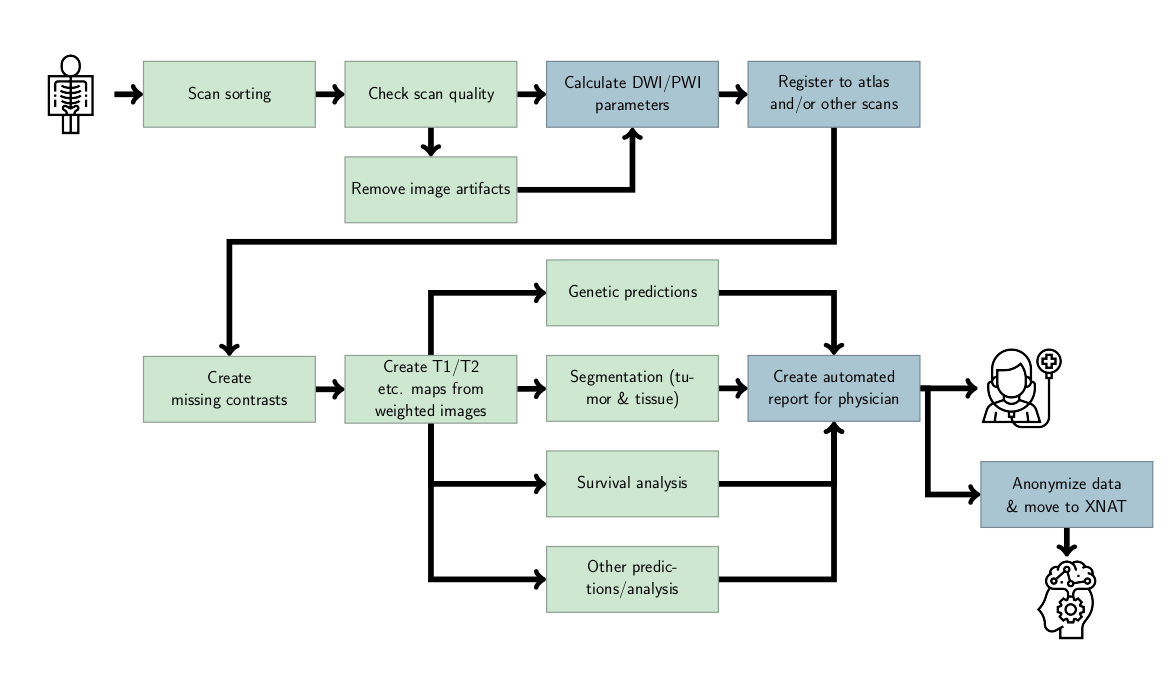
\includegraphics[width=\textwidth]{Figures/Pipeline.png}
\caption{Overview of some steps in which automated or machine learning methods can play a role from the scanner till the scan reaches the clinician}\label{fig:discussion_pipeline_automatic}
\end{figure}



\section{Conclusion}\label{sec:discussion_conclusion}


The above discussion raises several important questions that need to be addressed in future research.
Perhaps the most important question is what the future clinical application of radiomics will be.


First of all, the view in which radiomics is usually presented: to obviate the need for invasive or complicated surgery.
In the case of glioma, it seems unlikely that radiomics methods will completely replace biopsies or prevent surgeries.
The majority of the \glspl{tumor} are removed quickly after discovery, and the benefits of a watch-and-wait approach are often a topic of discussion.
As discussed in \cref{subsec:discussion_added_value_radiomics}, in this context radiomics method might need to focus on subgroups of patients for which they can provide the most benefits.

As mentioned above, radiomics can also be viewed as a way of democratizing the latest developments in glioma research.
This democratization would require models to be shared publicly, and requires guidelines on when and how these radiomics models can be used if no golden standard method is available.
These guidelines should be made as approachable as possible to ensure that the use of these models has a low threshold.

All in all, radiomics and automated image analysis are definitely here to stay.
With the increasing healthcare costs, the increasing amounts of data, and the decreasing amount of time clinical experts can spend on a single patient, automatic methods offer a cheap solution that can efficiently deal with large amounts of data.
Although several methodological and clinical barriers still need to be overcome, the ultimate goal of improved patient healthcare should be kept as the focus to guide future research.
Ultimately, we do need to move away from the human eye to more objective analysis methods, while at the same time making sure that these automated methods provide the information clinicians need, ensuring that they both play into each other's strengths.
